\documentclass[twoside]{article}
\usepackage{amsmath,amssymb,graphics,multirow,natbib}

\input{ISC18-english.sty}
\begin{document}
\thispagestyle{empty}
%%%%%%%%%%%%%%%%% Article title header  %%%%%%%%%%%%%%%%%%%%
\fancyhead[LE]{A Multivariate Risk Measure Under Linear Constraint}
%%%%%%%%%%%%%%%%% Article authors header   %%%%%%%%%%%%%%%%%%%%
\fancyhead[RO]{Roozegar and Mardani--Fard}
\begin{center}
{
\includegraphics [height=25mm, width=150.3mm] {Images/isc18E}} \\
\vspace*{-1.8cm}
%\begin{center}
%\color{blue} 
%{\hspace{0.1cm}\rule{\textwidth}{1mm}}\\
%\end{center}
\vspace*{4cm}
%%%%%%%%%%%%%%%%% Article title  %%%%%%%%%%%%%%%%%%%%
{\Large \bf Multivariate Tail Conditional Expectation Under a Linear
	Constraint: A New Risk Measure for Aggregated Exposures}\\
%%%%%%%%%%%%%%%%% Article authors and affiliations %%%%%%%%%%%%%%%%%%%%
{\bf
Roohollah Roozegar$^1$\footnote[2]{{\bf Corresponding Author:} {\tt roozegar@yu.ac.ir}}, Heydar Ali Mardani--Fard$^1$  \\
$^1$Department of Mathematics, Yasouj university, Yasouj, Iran
}
\end{center}
\rule{\textwidth}{0.2mm}\\
%%%%%%%%%%%%%%%%% Article abstract  %%%%%%%%%%%%%%%%%%%%
\noindent{\bf Abstract:}\\
Most multivariate tail risk measures, such as the multivariate tail
conditional expectation (MTCE), assume that all risk factors exceeds their
marginal quantiles simultaneously. But, in real word, this assumption
sometimes is unrealistic, since systemic events are typically generated by a
linear combination of risk factors crossing a critical threshold. So, in
this paper, we propose a new risk measure called the multivariate tail
conditional expectation under a linear constraint (MTCE-LC). This new risk
measure captures the expected risk conditional on a weighted sum of risk
factors exceeding a high quantile, so that weakness in one risk factor can
be offset by strength in another. This measure can be a good tool for stress
testing and capital allocation in systemic risk management. We present an
exact expression for the proposed measure under multivariate normal risk
factors and also, we carry out a Monte Carlo simulation study to show the
accuracy of the theoretical results.
 
\noindent{\bf Keywords:} 
Tail conditional expectation, Multivariate risk measure, Linear constraint, Systemic risk, Multivariate normal distribution. \\
\noindent{\bf Mathematics Subject Classification (2010):} $\rm 62H10$, $\rm 60E05$. \\
\hspace{1cm}\rule{\textwidth}{0.2mm}\\
%%%%%%%%%%%%%%
\section{Introduction}
As we know, a risk measure is a function from a set of random variables
associating the risks to a real number. In this regards, several risk
measures have been discussed in the literature, primarily used for
determining reserves needed for assets within the financial system. For a
single risk factor, one of the most important risk measures is the so-called
tail conditional expectation (TCE), which is the expected amount of the
worst losses, given the loss exceeds a certain quantile level. Let $X$ be a
loss random variable; then, the TCE is defined as%
\begin{equation*}
	TCE_{q}\left( X\right) =E\left( X\left\vert X>x_{q}\right. \right) ,~~q\in
	(0,1),
\end{equation*}%
where $x_{q}$ is a q-th quantile of the distribution of $X$, which is called
the value at risk (VaR) measure. It should be kept in mind that in many
applications, the risk managers encounter a set of risks instead of only one
risk. For example, in fields such as engineering, finance and insurance,
modeling joint risk factors plays a critical role in assessing portfolio
risks, pricing correlated assets and designing systems resilient to
simultaneous failures. To be specific, suppose the financial institution has 
$p$ different lines of businesses and $X=\left( X_{1},...,X_{p}\right) ^{T}$
is a vector of risks, where $X_{i}$ denotes the risk of the i-th business
line at the end of a specified period. In this regards, several works have
been carried out to extend the concept of tail risk measures from the
univariate case to the multivariate case; one may refer to \citet{Abbasi2013,Landsman2016,Roozegar2025}.

A popular way to extend the TCE measure to a multivariate framework is to
consider the total risk of the business lines. For this purpose, let $%
S=X_{1}+...+X_{p}$ denote the total risk of the $p$ business lines. Then,
the TCE of the random variable $S$ is defined as%
\begin{equation*}
	TCE_{q}\left( S\right) =E\left( S\left\vert S>s_{q}\right. \right) .~~
\end{equation*}

For a pair of risk factors $\mathbf{X}=(X_{1},X_{2})^{T}\in \lbrack 0,\infty
)^{2},$ with $E\left( X_{1}\right) <\infty ,$ \citet{Acharya2010} extended
the definition of TCE to the marginal expected shortfall (MES). This measure
is of the form 
\begin{equation*}
	MES_{q}\left( X_{1},X_{2}\right) =E\left( X_{1}\left\vert
	X_{2}>x_{2q}\right. \right) .
\end{equation*}%
The MES is a vital systemic risk measure utilized for assessing risk
contagion between two factors within a system. This measure has found
applications in finance and environmental science, as demonstrated by
studies of \citet{Caporin2012, Brownlees2015}.

\citet{Landsman2018} proposed a novel multivariate tail conditional
expectation (MTCE) under multivariate normal distribution risk facors, which
has several advantages. Let $\mathbf{X}\thicksim N_{p}\left( %
\mbox{\boldmath$\xi$},\mathbf{\Omega }\right) ~$be a vector of risks; then,
MTCE is defined as%
\begin{equation*}
	MTCE_{\mathbf{x}_{\mathbf{q}}}\left( \mathbf{X}\right) =E\left( \mathbf{X}%
	\left\vert \mathbf{X}>\mathbf{x}_{\mathbf{q}}\right. \right) =E\left( 
	\mathbf{X}\left\vert X_{1}>x_{1q_{1}},...,X_{p}>x_{pq_{p}}\right. \right) ,
\end{equation*}%
where $x_{\mathbf{q}}~$is a $q\times \ 1$ vector and $x_{iq_{i}}$ denotes
the $q_{i}$-th quantile of the marginal distribution of $X_{i}$, for $i\in
\{1,...,p\}$.

While the classical MTCE provides valuable information about joint tail
behavior, it has an important limitation: in many real world applications,
risk exposures are not independent, and a systemic risk event is often
triggered by a linear combination of risk factors exceeding a critical
threshold, rather than by each factor individually exceeding its own
quantile. For example, in a bank's portfolio, the total loss $%
L=c_{1}X_{1}+...+c_{p}X_{p}$ (with weight $c_{i}$ representing exposures)
may become critical even if some individual risks remain below their
quantiles. Similarly, in environmental risk assessment, the overall
pollution index --- a weighted sum of several pollutants --- may exceed a
regulatory limit without any single pollutant reaching its extreme quantile.
Therefore, in this paper, we introduce a new risk measure, called the
multivariate tail conditional expectation under a linear constraint
(MTCE-LC). We defined this measure as%
\begin{equation*}
	MTCE_{_{_{l_{q}}}}^{LC}\left( \mathbf{X}\right) =E\left( \mathbf{X}%
	\left\vert L>l_{q}\right. \right) ,
\end{equation*}%
where the risk vector $\mathbf{X~}$follows a multivariate normal
distribution with mean vector $\mbox{\boldmath$\xi$}$ and covarince matrix $%
\mathbf{\Omega }$, $\mathbf{c}=\left( c_{1},...,c_{p}\right) ^{T}~$ is a
vector of known weights, and $l_{q}~$denotes the q-th quantile of the
distribution of the linear combination $L=\mathbf{c}^{T}\mathbf{X.~}$This
measure captures the expected value of each risk factor conditional on the
total linear score exceeding a high threshold. Unlike the MTCE measure,
which requires simultaneous exceedances of all marginals, the proposed
MTCE-LC allows for compensatory effects between risk factors, making it more
flexible and realistic for systemic risk monitoring, capital allocation, and
stress testing. Furthermore, when $p=1$ ans $c=1$, the proposed measure
reduces to the univariate TCE, ensuring consistency with previous risk
measures.

\section{MTCE-LC for multivariate normal risk scenarios}

This section focuses on obtaining an exact expression for MTCE-LC within the
class of multivariate normal distribution. For this purpose, we need to
derive the expectation of the multivarite truncated normal distribution
where truncation is based on a single linear combination of the variables,
which we denote by MTN-LC (Multivariate Truncated Normal -- Linear
Combination). We denote this model by $\mathbf{Y}=\mathbf{X}\left\vert a<%
\mathbf{c}^{T}\mathbf{X}<b,\right. $ where $\mathbf{X}\thicksim N_{p}\left( %
\mbox{\boldmath$\xi$},\mathbf{\Omega }\right) .$

Over the last five decades, several works have appeared in the literature
discussing the computation of expectations for the truncated multivariate
normal distribution; see for example, \citet{Tallis1961, Lee1979, Horrace2005, Ho2012,Roozegar2020}.
But, these classical results assume that each coordinate of the multivariate normal vector is
truncated independently within a hyper-rectangle. In this section, we
considers a fundamentally different scenario where truncation based on a
single linear combination of variables and derive an exact expression for
the mean of this distribution. For this purpose, First, we derive the
probability density function (pdf) of a univariate component of a standard
MTN-LC, which we need for subsequent derivation.

Let $c_{i}$, for $i=1,...,p$, denote the i-th component of a $p$-dimensional
vector $c=\left( c_{1},...,c_{p}\right) ^{\top },$ and by $c_{-i}$ the
vector obtained from $c$ by deleting its i-th component. Furthermore, for
the standard univariate normal distribution, let $\phi \left( .\right) $ and 
$\Phi \left( .\right) $ denote its pdf and cumulative distribution function
(cdf), respectively, and $\overset{\_}{\Phi }\left( a,b\right) $ be the
probability in real line $\left( a,b\right) $. Then we have the following
lemma.

\begin{lem}\label{lem1}
	Let $Z\thicksim N_{p}\left( \mathbf{0},\mathbf{I}%
_{p}\right) $, and for $i\in \left\{ 1,...,p\right\} $, define $Y_{i}\overset%
{d}{=}Z_{i}\mathbf{\mid }\left( a\mathbf{<c}^{T}\mathbf{Z<}b\right) .$ Then,
the pdf of univariate random variable $Y_{i}$ can be derived as%
\begin{equation*}
	f_{Y_{i}}\left( y_{i}\right) =\frac{\phi \left( y_{i}\right) }{\overset{\_}{%
			\Phi }\left( \frac{a}{\sqrt{\mathbf{c}^{T}\mathbf{c}}},\frac{b}{\sqrt{%
				\mathbf{c}^{T}\mathbf{c}}}\right) }\left\{ \Phi \left( \lambda
	_{i}y_{i}+\tau _{i}^{b}\right) -\Phi \left( \lambda _{i}y_{i}+\tau
	_{i}^{a}\right) \right\} ,
\end{equation*}%
where%
\begin{equation*}
	\lambda _{i}=-\frac{c_{i}}{\sqrt{\mathbf{c}_{\mathbf{-}i}^{T}\mathbf{c}_{-i}}%
	},~\tau _{i}^{a}=\frac{a}{\sqrt{\mathbf{c}_{\mathbf{-}i}^{T}\mathbf{c}_{-i}}}%
	\text{ and }\tau _{i}^{b}=\frac{b}{\sqrt{\mathbf{c}_{\mathbf{-}i}^{T}\mathbf{%
				c}_{-i}}}.
\end{equation*}%
\end{lem}

\begin{proof}
We can write the random variable $Y_{i}$ as 
\begin{equation*}
	Y_{i}\overset{d}{=}Z_{i}\mathbf{\mid }\left( a-c_{i}Z_{i}\mathbf{<\mathbf{c}%
		_{\mathbf{-}i}^{T}Z}_{-i}\mathbf{<}b-c_{i}Z_{i}\right) .
\end{equation*}%
Then, using Bayes' theorem, we can write the pdf of $Y_{i}$ as 
\begin{equation*}
	f_{Y_{i}}\left( y_{i}\right) =\frac{\Pr \left( a-c_{i}y_{i}\mathbf{<\mathbf{c%
			}_{\mathbf{-}i}^{T}Z}_{-i}\mathbf{<}b-c_{i}y_{i}\right) \phi \left(
		y_{i}\right) }{\Pr \left( a\mathbf{<c}^{T}\mathbf{Z<}b\right) },
\end{equation*}%
which yields the desired result.
\end{proof}

\begin{thm}\label{thm1}
	Let $\mathbf{X}\thicksim N_{p}\left( %
\mbox{\boldmath$\xi$},\mathbf{\Omega }\right) ,$ and define $\mathbf{Y}%
\overset{d}{=}\mathbf{X\mid }\left( a\mathbf{<c}^{T}\mathbf{X<}b\right) .$
Then, the first moments of random vector $\mathbf{Y}$ can be obtained as%
\begin{equation*}
	E\left( \mathbf{Y}\right) =\mbox{\boldmath$\xi$}+\mathbf{Bq}\left( a^{\ast
	},b^{\ast },\mathbf{c}^{\ast }\right) ,
\end{equation*}%
where $\mathbf{BB}^{T}\mathbf{=\Omega }$ and the i-th element of the $%
p\times \ 1$ vector $\mathbf{q}\left( a^{\ast },b^{\ast },\mathbf{c}^{\ast
}\right) $ is%
\begin{equation*}
	q_{i}\left( a^{\ast },b^{\ast },\mathbf{c}^{\ast }\right) =\frac{c_{i}^{\ast
	}}{\sqrt{\mathbf{c}^{\ast ^{T}}\mathbf{c}^{\ast }}}\frac{1}{\overset{\_}{%
			\Phi }\left( \frac{a^{\ast }}{\sqrt{\mathbf{c}^{\ast ^{T}}\mathbf{c}^{\ast }}%
		},\frac{b^{\ast }}{\sqrt{\mathbf{c}^{\ast ^{T}}\mathbf{c}^{\ast }}}\right) }%
	\left[ \phi \left( \frac{a^{\ast }}{\sqrt{\mathbf{c}^{\ast ^{T}}\mathbf{c}%
			^{\ast }}}\right) -\phi \left( \frac{b^{\ast }}{\sqrt{\mathbf{c}^{\ast ^{T}}%
			\mathbf{c}^{\ast }}}\right) \right] ,
\end{equation*}%
with
\begin{equation}
	a^{\ast }=a-\mathbf{c}^{T}\mbox{\boldmath$\xi$},~b^{\ast }=b-\mathbf{c}^{T}%
	\mbox{\boldmath$\xi$},~\text{and}~\mathbf{c}^{\ast }=\mathbf{B}^{T}\mathbf{c}%
	.  \label{e1}
\end{equation}
\end{thm} 

\begin{proof}
First, let $\mathbf{Z}\thicksim
N_{p}\left( \mathbf{0},\mathbf{I}\right) $, and $\mathbf{Y}\overset{d}{=}%
\mathbf{Z\mid }\left( a\mathbf{<c}^{T}\mathbf{Z<}b\right) .$ From the result
in Lemma 1, we have%
\begin{equation*}
	E\left( Y_{i}\right) =\frac{1}{\overset{\_}{\Phi }\left( \frac{a}{\sqrt{%
				\mathbf{c}^{T}\mathbf{c}}},\frac{b}{\sqrt{\mathbf{c}^{T}\mathbf{c}}}\right) }%
	\int_{-\infty }^{+\infty }y_{i}\phi \left( y_{i}\right) \left\{ \Phi \left(
	\lambda _{i}y_{i}+\tau _{i}^{b}\right) -\Phi \left( \lambda _{i}y_{i}+\tau
	_{i}^{a}\right) \right\} dy_{i}.
\end{equation*}%
Using integration by parts and simplifying, we obtain 
\begin{eqnarray*}
	\int_{-\infty }^{+\infty }y_{i}\phi \left( y_{i}\right) \Phi \left( \lambda
	_{i}y_{i}+\tau _{i}^{b}\right) dy_{i} &=&\lambda _{i}\int_{-\infty
	}^{+\infty }\phi \left( y_{i}\right) \phi \left( \lambda _{i}y_{i}+\tau
	_{i}^{b}\right) dy_{i} \\
	&=&\frac{\lambda _{i}}{\sqrt{1\mathbf{+}\lambda _{i}^{2}}}\phi \left( \frac{%
		\tau _{i}^{b}}{\sqrt{1\mathbf{+}\lambda _{i}^{2}}}\right) \int_{-\infty
	}^{+\infty }\phi \left( y_{i};-\frac{\lambda _{i}\tau _{i}^{b}}{1\mathbf{+}%
		\lambda _{i}^{2}},\frac{1}{1\mathbf{+}\lambda _{i}^{2}}\right) dy_{i} \\
	&=&-\frac{c_{i}}{\sqrt{\mathbf{c}^{T}\mathbf{c}}}\phi \left( \frac{b}{\sqrt{%
			\mathbf{c}^{T}\mathbf{c}}}\right) .
\end{eqnarray*}%
Therefore, in the standard case, 
\begin{equation*}
	E\left( Y_{i}\right) =\frac{c_{i}}{\sqrt{\mathbf{c}^{T}\mathbf{c}}}\frac{1}{%
		\overset{\_}{\Phi }\left( \frac{a}{\sqrt{\mathbf{c}^{T}\mathbf{c}}},\frac{b}{%
			\sqrt{\mathbf{c}^{T}\mathbf{c}}}\right) }\left[ \phi \left( \frac{a}{\sqrt{%
			\mathbf{c}^{T}\mathbf{c}}}\right) -\phi \left( \frac{b}{\sqrt{\mathbf{c}^{T}%
			\mathbf{c}}}\right) \right] .
\end{equation*}%
For the general case, when $\mathbf{X}\thicksim N_{p}\left( %
\mbox{\boldmath$\xi$},\mathbf{\Omega }\right) $, we have $\mathbf{X}\overset{%
	d}{=}\mbox{\boldmath$\xi$}+\mathbf{BZ,}$ where $\mathbf{Z}\thicksim
N_{p}\left( \mathbf{0},\mathbf{I}\right) $ and $\mathbf{BB}^{T}\mathbf{%
	=\Omega .}$ So, the random vector $\mathbf{Y}\overset{d}{=}\mathbf{X\mid }%
\left( a\mathbf{<c}^{T}\mathbf{X<}b\right) $ can be written as 
\begin{eqnarray*}
	&&\mathbf{Y}\overset{d}{=}\mbox{\boldmath$\xi$}+\mathbf{BZ\mid }a\mathbf{<c}%
	^{T}\left( \mbox{\boldmath$\xi$}+\mathbf{BZ}\right) \mathbf{<}b \\
	&&\overset{d}{=}\mbox{\boldmath$\xi$}+\mathbf{B}\left[ \mathbf{Z\mid }a-%
	\mathbf{c}^{T}\mbox{\boldmath$\xi$}\mathbf{<c}^{T}\mathbf{BZ<}b-\mathbf{c}%
	^{T}\mbox{\boldmath$\xi$}\right] .
\end{eqnarray*}%
Letting $a^{\ast },~b^{\ast }~$and$~\mathbf{c}^{\ast }\ $as in (\ref{e1})$%
\mathbf{,}$ we obtain%
\begin{equation*}
	E\left( \mathbf{Y}\right) =\mbox{\boldmath$\xi$}+\mathbf{B}E\left( \mathbf{%
		Z\mid }a^{\ast }\mathbf{<}\left( \mathbf{c}^{\ast }\right) ^{T}\mathbf{Z<}%
	b^{\ast }\right) ,
\end{equation*}%
which, using the standard-case result above, gives the expression in the
theorem.
\end{proof}

The MTCE-LC expression follows directly from Theorem 1 by letting $a$ = $%
l_{q}$ and $b$ tend to infinity. We present this result in the following
lemma.

\begin{lem}\label{lem2}
	If $\mathbf{X}\thicksim N_{p}\left( %
\mbox{\boldmath$\xi$},\mathbf{\Omega }\right) ,$ then 
\begin{equation*}
	MTCE_{_{_{l_{q}}}}^{LC}\left( \mathbf{X}\right) =\mbox{\boldmath$\xi$}+%
	\mathbf{Bq}\left( l_{q},\mathbf{c}^{\ast }\right)
\end{equation*}%
where $\mathbf{c}^{\ast }$ is defined as in (\ref{e1}) and the i-th element
of the $p\times \ 1$ vector $\mathbf{q}\left( l_{q},\mathbf{c}^{\ast
}\right) $ is%
\begin{equation*}
	q_{i}\left( l_{q},\mathbf{c}^{\ast }\right) =\frac{c_{i}^{\ast }}{\sqrt{%
			\mathbf{c}^{\ast ^{T}}\mathbf{c}^{\ast }}}\frac{1}{1-\Phi \left( \frac{l_{q}-%
			\mathbf{c}^{T}\mbox{\boldmath$\xi$}}{\sqrt{\mathbf{c}^{\ast ^{T}}\mathbf{c}%
				^{\ast }}}\right) }\phi \left( \frac{l_{q}-\mathbf{c}^{T}\mbox{\boldmath$%
			\xi$}}{\sqrt{\mathbf{c}^{\ast ^{T}}\mathbf{c}^{\ast }}}\right) .
\end{equation*}
\end{lem}

\section{Numerical illustration}

In this section, we present a Monte Carlo study to assess the accuracy of the
theoretical results derived in Lemma~\ref{lem1} and Theorem~\ref{thm1}. The simulation study is
conducted in two parts. In the first part, we examine the marginal densities of
the components of the truncated normal vector under a linear constraint and
compare the theoretical densities obtained from Lemma~\ref{lem1} with kernel density
estimates based on simulated samples. In the second part, we investigate the
accuracy of the theoretical expression for the mean vector given in Theorem 1 by
comparing it with empirical averages computed from simulated truncated samples.

\subsection{Assessment of Lemma~\ref{lem1}}

We first study the validity of Lemma~\ref{lem1} for the marginal distributions of the
components of the truncated vector
\[
\mathbf{Y} \overset{d}{=} \mathbf{Z}\mid \left(a < \mathbf{c}^\top \mathbf{Z} < b\right),
\]
where \(\mathbf{Z}\) is trivariate standard normal. In this part, we take
\[
\mathbf{c}=(-0.4,\,0.7,\,0.2)^\top.
\]
The truncation points \(a\) and \(b\) are chosen from quantiles of the linear
combination \(\mathbf{c}^\top\mathbf{Z}\) under two settings:
\[
(q_1,q_2)=(0.30,0.60), \qquad (q_1,q_2)=(0.80,0.95).
\]
Thus, the first setting corresponds to a moderate central truncation interval,
while the second one represents a more upper-tail and asymmetric truncation
region.

For each truncation setting, we generated \(10{,}000\) observations from the
corresponding truncated distribution and then estimated the marginal densities
of \(Y_1\), \(Y_2\), and \(Y_3\) by kernel smoothing using the \texttt{density}
function in \textsf{R}. These empirical densities were then compared with the
corresponding theoretical densities obtained from Lemma~\ref{lem1}.

Figure~\ref{fig:densities} displays the results. The figure is arranged in a
\(3\times 2\) layout: the rows correspond to the components \(Y_1\), \(Y_2\),
and \(Y_3\), while the two columns correspond to the two choices of the
truncation interval \((a,b)\). In each panel, the solid curve represents the
theoretical density, whereas the dashed curve represents the kernel density
estimate based on the simulated sample.

The agreement between the theoretical and empirical curves is remarkably close
in all cases. This confirms that the marginal density formula given in Lemma 1
provides an accurate description of the univariate components of the
multivariate normal distribution truncated by a linear constraint. The fit
remains very good both for the moderate truncation interval and for the more
extreme upper-tail truncation case, which provides strong numerical support for
the lemma.

\begin{figure}[ht]
	\begin{center}
	\includegraphics[width=0.9\textwidth]{Images/Plot_Densities.eps}
	\vspace{-0.2cm}
	\caption{\footnotesize Comparison between the theoretical marginal densities from Lemma~1 and
		the kernel density estimates obtained from \(10{,}000\) simulated observations
		from the trivariate truncated normal distribution under a linear constraint. The
		rows correspond to \(Y_1\), \(Y_2\), and \(Y_3\), and the columns correspond to
		the two truncation settings determined by the quantile pairs
		\((0.30,0.60)\) and \((0.80,0.95)\) of \(\mathbf{c}^\top \mathbf{X}\), with
		\(\mathbf{c}=(-0.4,0.7,0.2)^\top\). In each panel, the solid line denotes the
		theoretical density and the dashed line denotes the simulation-based kernel
		density estimate.}
	\label{fig:densities}
	\end{center}
\end{figure}

\subsection{Assessment of Theorem~\ref{thm1}}

We next evaluate the theoretical expression for the mean vector given in
Theorem~\ref{thm1}. In this part, we take the mean vector of the original multivariate
normal distribution as
\[
\boldsymbol{\xi}=(1,1,1)^\top,
\]
and the coefficient vector in the linear constraint as
\[
\mathbf{c}=(0.2,0.3,0.4)^\top.
\]
We consider three covariance structures:
\[
\Sigma_1=
\begin{pmatrix}
	1 & 0 & 0\\
	0 & 1 & 0\\
	0 & 0 & 1
\end{pmatrix},
\qquad
\Sigma_2=
\begin{pmatrix}
	1 & 0.5 & 0.5\\
	0.5 & 1 & 0.5\\
	0.5 & 0.5 & 1
\end{pmatrix},
\]
and
\[
\Sigma_3=
\begin{pmatrix}
	1.0 & 0.75 & 0.0\\
	0.75 & 1.2 & -0.55\\
	0.0 & -0.55 & 0.8
\end{pmatrix}.
\]

For the truncation interval, we again use quantiles of the linear combination
\(\mathbf{c}^\top \mathbf{X}\). Two cases are considered:
\[
\text{Case 1: } (q_1,q_2)=(0.20,0.80), \qquad
\text{Case 2: } (q_1,q_2)=(0.40,0.85).
\]
The first case corresponds to a symmetric central truncation interval, while
the second one corresponds to a more asymmetric interval. For each covariance
structure and each truncation case, we computed the theoretical mean vector
using the formula in Theorem~\ref{thm1} and compared it with the empirical mean obtained
from \(10^6\) simulated observations from the corresponding truncated normal
distribution.

The results are reported in Table~\ref{tab:meancomp}. The numerical agreement
between the theoretical and simulated values is excellent across all three
components, all covariance structures, and both truncation settings. The
differences are negligible and can be attributed to Monte Carlo error. These
results provide clear numerical confirmation of Theorem~\ref{thm1} and show that the
proposed expression for the mean vector of the linearly truncated multivariate
normal distribution is highly accurate.

\begin{table}[ht]
	\begin{center}
		\small
	\caption{Theoretical and simulated componentwise means of the truncated trivariate normal distribution under the linear constraint \(a<\mathbf{c}^\top\mathbf{X}<b\), for \(\boldsymbol{\xi}=(1,1,1)^\top\), \(\mathbf{c}=(0.2,0.3,0.4)^\top\), and three covariance structures. Case 1 corresponds to the quantile pair \((0.20,0.80)\), and Case 2 corresponds to \((0.40,0.85)\). Simulated values are based on \(10^6\) generated observations.}
	\label{tab:meancomp}
	\begin{tabular}{cccccccc}
		\hline
		&  & \multicolumn{2}{c}{\(\Sigma_1\)} & \multicolumn{2}{c}{\(\Sigma_2\)} & \multicolumn{2}{c}{\(\Sigma_3\)} \\
		\cline{3-8}
		Case & Component & Theo. & Sim. & Theo. & Sim. & Theo. & Sim. \\
		\hline
		\multirow{3}{*}{Case 1}
		& \(Y_1\) & 0.4999 & 0.4996 & 0.2828 & 0.2821 & -0.3238 & -0.3249 \\
		& \(Y_2\) & 0.2498 & 0.2501 & 0.2176 & 0.2179 & 0.0967 & 0.0959 \\
		& \(Y_3\) & -0.0003 & -0.0004 & 0.1524 & 0.1519 & 0.5172 & 0.5182 \\
		\hline
		\multirow{3}{*}{Case 2}
		& \(Y_1\) & 0.5846 & 0.5831 & 0.4690 & 0.4693 & -0.1299 & -0.1304 \\
		& \(Y_2\) & 0.3769 & 0.3771 & 0.4207 & 0.4207 & 0.2290 & 0.2292 \\
		& \(Y_3\) & 0.1693 & 0.1697 & 0.3724 & 0.3725 & 0.5879 & 0.5887 \\
		\hline
	\end{tabular}
	\end{center}
\end{table}

Overall, the simulation study strongly supports the theoretical developments of
this paper. The density comparisons verify the marginal distributional result
in Lemma~1, while the numerical agreement between theoretical and empirical
mean vectors confirms the validity of Theorem~\ref{thm1}. Hence, the proposed formulas
provide an accurate and practically useful framework for analyzing multivariate
normal risks under linear truncation constraints.

\section*{Discussion and Conclusion}   
In this paper, we have proposed a modified version of the MTCE measure,
called MTCE-LC, which solve a limitation of MTCE measure by conditioning on a
weighted sum of risk factors exceeding a high quantile rather than requiring
simultaneous exceedances of all marginal quantiles. We have illustrated the
accuracy of the results using a numericl illustration. It will, of course, be
of interest to look for such measures for the class of elliptical,
skew-elliptical and scale-mixtures of multivariate normal distributions and
we are currently looking into this problem and hope to report the findings
in a future paper.
%\section*{Acknowledgments}   

\begin{thebibliography}{99}
	\bibitem[Abbasi and Hosseinifard(2013)]{Abbasi2013} Abbasi, B., Hosseinifard., S. Z. (2013). Tail conditional
	expectation for multivariate distributions: A game theory approach,
	Statistics \& Probability Letters, 83, 2228--2235.
	
	\bibitem[Acharya et al.(2010)]{Acharya2010} Acharya, V.V., Pedersen, L.H., Philippon, T., Richardson, M.
	(2010). Measuring systemic risk. FRB of Cleveland Working Paper No. 10-02.
	https://ssrn.com/abstract=1595075.
	
	\bibitem[Brownlees and Engle(2015)]{Brownlees2015} Brownlees, C., Engle, E. (2015). SRISK: A conditional capital
	shortfall index for systemic risk management. The Review of Financial
	Studies, 30(1), 48-79.
	
	\bibitem[Caporin and Santucci(2012)]{Caporin2012} Caporin, M., Santucci de Magistris, P. (2012). On the evaluation
	of marginal expected shortfall. Applied Economics Letters, 19(2), 175-179.
	
	\bibitem[Ho et al.(2012)]{Ho2012} Ho, H. J., Lin, T. I., Chen, H. Y., Wang, W. L. (2012). Some
	results on the truncated multivariate t-distribution, Journal of Statistical
	Planning and Inference, 142, 25-40.
	
	\bibitem[Horrace(2005)]{Horrace2005} Horrace, W. C. (2005). Some results on the multivariate truncated
	normal distribution. Journal of Multivariate Analysis, 94(1), 209--221.
	
	\bibitem[Lee(1979)]{Lee1979} Lee, L. F. (1979). On the first and second moments of the
	truncated multi-normal distribution and a simple estimator. Economics
	Letters, 3(2), 165--169.
	
	\bibitem[Landsman et al.(2016)]{Landsman2016} Landsman, Z., Makov, U., Shushi, T. (2016) Multivariate tail conditional expectation for elliptical distributions, Insurance: Mathematics and Economics, 70, 216--223
	
	\bibitem[Landsman et al.(2018)]{Landsman2018} Landsman, Z., Makov, U., Shushi, T. (2018). A multivariate tail
	covariance measure for elliptical distributions, Insurance: Mathematics and
	Economics, 81, 27--35.
	
	\bibitem[Roozegar et al.(2020)]{Roozegar2020} Roozegar, R., Balakrishnan, N., Jamalizadeh, A. (2020). On
	moments of doubly truncated multivariate normal mean--variance mixture
	distributions with application to multivariate tail conditional expectation.
	Journal of Multivariate Analysis, 177, 104586.
	
	\bibitem[Roozegar et al.(2025)]{Roozegar2025} Roozegar, R., Balakrishnan, N., Mardani-Fard, H. A., Desmond, A.
	F., Jamalizadeh, A. (2025). Expressions for Marginal Mean Excess and
	Marginal Expected Shortfall Measures under Bivariate Scale Mixture of Normal
	Distribution. Methodology and Computing in Applied Probability, 27, 30.
	
	\bibitem[Tallis(1961)]{Tallis1961} Tallis, G. M. (1961). The moment generating function of the
	truncated multi-normal distribution. Journal of the Royal Statistical
	Society, Series B, 23, 223--229.
\end{thebibliography}
 \end{document}

